\documentclass[10pt]{article}
\usepackage[margin=.76 in]{geometry}
\usepackage{amsmath,amssymb,booktabs,graphicx,url,microtype,array}
\usepackage[T1]{fontenc}\usepackage[colorlinks=true,allcolors=blue]{hyperref}
\setlength{\parindent}{0 pt}\setlength{\parskip}{5 pt}
\begin{document}
\begin{center}{\Large\bfseries Finite-cell thermodynamics, path stability,\\and harmonic estimator diagnostics}\par\vspace{5 pt}
ECE 285 research supplement --- interim, November 8,2026\\
Ricardo Silva Buarque, Beihao Gu, and Varad Kottawar
\end{center}
This supplement separates three questions from the class generator comparison:
what a small finite static model predicts exactly, whether a saved migration
path is numerically stable, and how a thermal estimator behaves on a known
harmonic signal. Completed negative results are retained. No new DFT, MD event
search, MLIP fine-tuning or physical activation free-energy calculation occurs.

\section{Exact enumeration on the literal Hu 12-site parent}
The stored Li$_{12}$Co$_{12}$O$_{24}$ parent is an optimized Hu frame, not an ideal
symmetrized crystal. Its 144 retained Li-site permutations were accepted at
$0.001$~\AA\ coordinate tolerance; the maximum species-matching residual is
$0.000263895$~\AA. The complete combinatorial grouping has 87 orbits over all
counts. At 3/6/9 present Li it has 6/17/6 orbits containing 220/924/220 raw masks.
Those counts are exact for the retained permutation action, but the literal
coordinate Hamiltonian need not be exactly invariant under it.

Accordingly, every one of the 1,364 raw geometries was physically evaluated with
both UMA-S-1.2.1/\texttt{omat} and MACE-MH-1/\texttt{omat\_pbe}, FP32/TF32 off,
without relaxation. Two fixed masks per composition each received two additional
evaluations: 1,376 calls per teacher, 2,752 total, 0 failures. An evaluation retains
literal parent coordinates/species/cell and deletes the selected Li. A raw ID
and geometry hash identify that actual geometry; an orbit key is separate.
The stored historical representative mask, rather than a geometry inferred from
its canonical-code ID, selects the representative approximation.

At a fixed teacher and count, let $E_i$ be total-cell potential energy in eV,
$M$ the number of raw states, $T$ temperature in K and
$k_B=8.617333262145\times 10^{-5}$~eV/K. With
$\beta=1/(k_BT)$ and $E_0=\min_iE_i$,
\begin{align}
Z_{\rm rel}&=\sum_{i=1}^M e^{-\beta(E_i-E_0)},&
p_i&=e^{-\beta(E_i-E_0)}/Z_{\rm rel},\\
\langle E\rangle&=\sum_i p_iE_i,&
S&=-k_B\sum_i p_i\log p_i,\\
F&=E_0-k_BT\log Z_{\rm rel}=\langle E\rangle-TS.
\end{align}
$p_i$ is dimensionless; $S$ has eV/K per simulated cell. The normalization is
separate for each composition: no lithium chemical-potential ensemble is implied.
The exact-reference effective state count $1/\sum_i p_i^2$ measures concentration
of this finite distribution, not reliability of an MD sample.

For group $a$, $g_a$ counts its raw members and $P_a=\sum_{i\in a}p_i$ is its
probability. The exact entropy identity is
\begin{equation}
S=-k_B\sum_aP_a\log P_a+\sum_a P_a S(i\mid a),\quad
S(i\mid a)=-k_B\sum_{i\in a}\frac{p_i}{P_a}\log\frac{p_i}{P_a}.
\end{equation}
Only equal-energy members give $S(i\mid a)=k_B\log g_a$ and therefore
$S=-k_B\sum_aP_a\log(P_a/g_a)$. Keeping only $-\sum P_a\log P_a$ drops
within-orbit entropy. This identity was checked under an exactly symmetric null
and independently on the raw data; no CVAE latent entropy is involved.
\newpage

\subsection{Measured approximate symmetry and teacher disagreement}
The largest within-orbit energy ranges are 2.730 meV/cell for UMA and 2.777 for MACE.
Maximum repeated-identical-geometry ranges are 0.00650 and 0.01526 meV/cell,
respectively. Thus approximate symmetry is detectably inexact beyond repeat
noise. Its effect on representative-weight thermodynamics is nevertheless small
here: at 433.15 K the largest orbit-probability total variation is 0.00176.
This empirical smallness is not permission to assume equality in another parent.

\begin{center}\small
\begin{tabular}{crrrrr}\toprule
Li count&Raw/orbits&$S_{\rm U}/k_B$&$S_{\rm M}/k_B$&$N_{\rm eff,U}$&$N_{\rm eff,M}$\\\midrule
3&220/6&4.1758&4.1665&63.38&63.99\\
6&924/17&4.3958&5.3783&33.99&212.59\\
9&220/6&3.1213&4.1328&11.09&60.67\\\bottomrule
\end{tabular}
\end{center}
Here U/M denote UMA/MACE, and all values are at 433.15 K. The entropy difference
at half filling is therefore mainly teacher dependence, rather than the small
representative-weight approximation error. The teachers select different
lowest \emph{mean-energy orbits} at every count. Their group-mean energy rank
Spearman coefficients are 0.714/0.814/0.714 at 3/6/9 Li, respectively. Raw rank
coefficients are lower(approximately 0.54/0.51/0.54) and also include the ordering
of nearly degenerate members inside an approximate orbit. Neither analysis
identifies which teacher is closer to DFT.

\begin{center}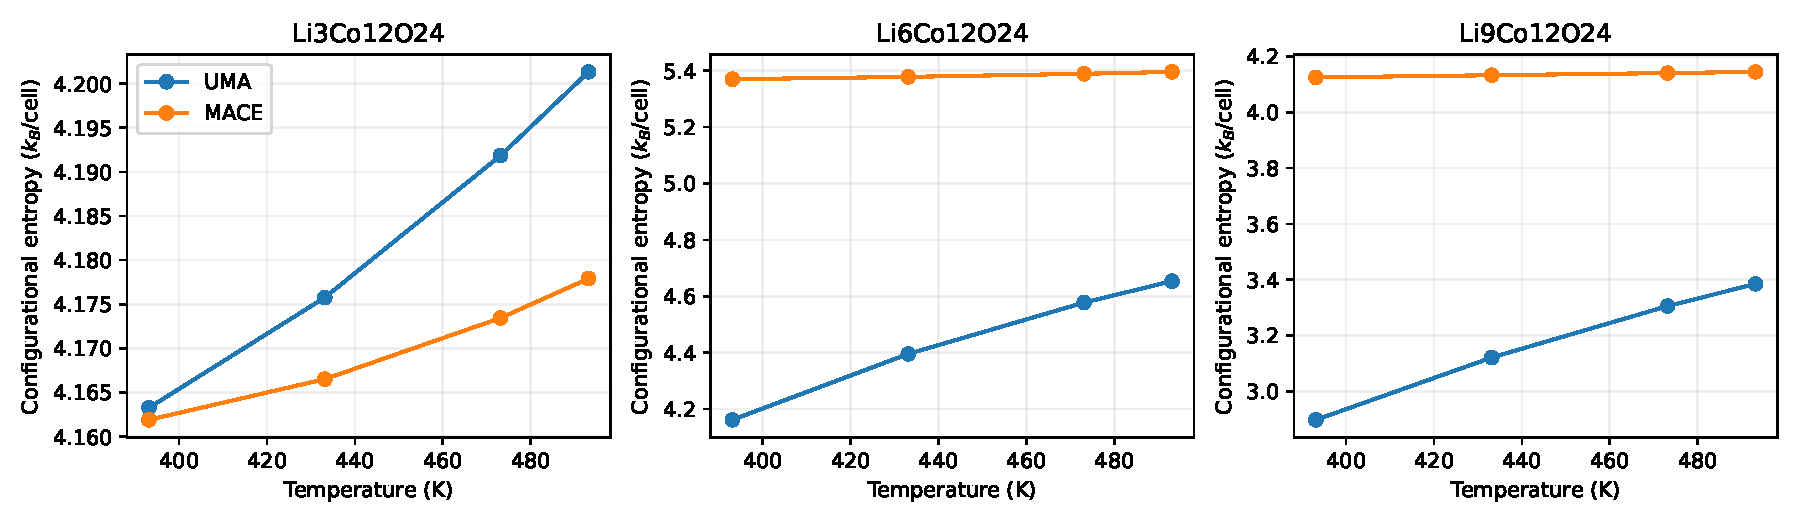
\includegraphics[width=.96\linewidth]{assets/finite_entropy.pdf}\end{center}
\textbf{Finite-reference pool errors.} A uniform-raw IID pool with replacement
contains $L$ draws $I_1,\ldots,I_L$ from the known universe of $M$ states. Its
partition estimator is
\begin{equation}
\widehat Z_{\rm rel}=\frac{M}{L}\sum_{\ell=1}^L e^{-\beta(E_{I_\ell}-E_0)},\quad
\widehat S=k_B[\log\widehat Z_{\rm rel}+\beta(\widehat{\langle E\rangle}-E_0)].
\end{equation}
The normalized sample weights form $\widehat{\langle E\rangle}$. The partition
estimate is unbiased under this sampling law; its logarithm and resulting
energy/entropy estimates need not be. Repeated raw draws retain their particle
multiplicity; adding symmetry multiplicities again would double count.
Five seeds and nested 32/64/128/256/512/1,024 draw budgets quantify error,
probability mass covered, bin-mass error and particle ESS. A proposal-histogram
entropy would answer another question. Nested budgets share random draws and
are not independent replicates. This is finite static-model validation only;
it neither validates a 48-site model on 12 sites nor estimates real-LCO entropy.
\newpage

\section{NEB: fixed endpoints, route initialization and numerical stability}
The nudged elastic band(NEB) method connects given endpoints using a chain of
interior atomistic images. Physical forces perpendicular to the chain relax the
route, while artificial springs distribute images. A climbing image reverses
the force component along the local path tangent to seek a maximum along that
direction \cite{aseNEB}. Its projected-force stopping criterion differs from the
physical force at ordinary nonclimbing images; those images are not expected
to be individual local minima.

Two saved MD events retain continuous atom identities and periodic branches.
The marked event 1 Li is local atom 65(parent 66), moving between parent Li sites
18 and 31; event 2 is local/parent atom 59, between sites 11 and 23 with periodic image
$(1,0,0)$. The ideal-site displacement in each is 2.8113\AA. Independent
canonicalization of endpoints would destroy this event information; an event
can be real even if its endpoint occupation orbits are symmetry-equivalent.

The first tranche held the exact old endpoint coordinates and cell fixed,
resampled the saved route families to seven interior images, and used the common
$0.02$~eV/\AA\ projected-force target. ASE 3.26.0, improved tangent, climbing image,
$k=0.1$~eV/\AA$^2$, FIRE $dt=0.1$, $dt_{\max}=1$, maximum step 0.05\AA,
serial images sharing one GPU backend through independent caches, and no new
IDPP/event search were declared. Each band is capped at 500 optimizer steps,
45 minutes including imports/loading, and 5,000 actual E/F/stress calls.

\begin{center}\small
\begin{tabular}{p{.35\linewidth}rrr}\toprule
Case&Steps&Projected max force&Terminal forward span\\
& &eV/\AA&eV/hop\\\midrule
Event 1 coarse route, 7 interior&500&0.2253&0.2468(not converged)\\
Event 1 refined route, 7 interior&430+interruption&0.8877&not a barrier estimate\\
Event 1 bounded recovery&69&0.4929&0.2433(not converged)\\
Event 1 old 7 exact coordinates&500&0.3471&0.2493(not converged)\\
Event 2,5 interior&11&0.01338&0.17598\\
Event 2,7 interior&21&0.01997&0.17702\\
Event 2,9 interior&33&0.01999&0.17237\\\bottomrule
\end{tabular}
\end{center}
The original event 1 refined worker was externally killed by Slurm fail-fast when
its sibling reached the scientific step cap. Its 430-step snapshot and 3,020
successful calls are preserved. One additional in-flight position update is
conservatively charged: only 69 of the original 500 steps remain. Recovery restores
that exact snapshot, resets FIRE memory explicitly, and preserves the original
time/call reservation; it is not a fresh 500-step rerun. Equal-arclength resampling
redistributes even an already-seven-image band, so an additional declared
direct-coordinate continuation tested that initialization difference. It too
hit the 500-step cap. Resampling alone therefore does not explain the failure.

The event 2 forward-span spread across 5/7/9 interior images is 0.00465 eV/hop, below
the predeclared 0.02 eV/hop practical numerical target. This is a chosen numerical
criterion, not model/DFT accuracy. Event 1 remains unresolved; convenient terminal
spans must not be selected as validated barriers. Event 2 endpoint physical forces
remain 0.02954/0.01264 eV/\AA\ because the endpoints were held fixed. Numerical
image stability is conditional on those endpoints and that potential.
\newpage

\begin{center}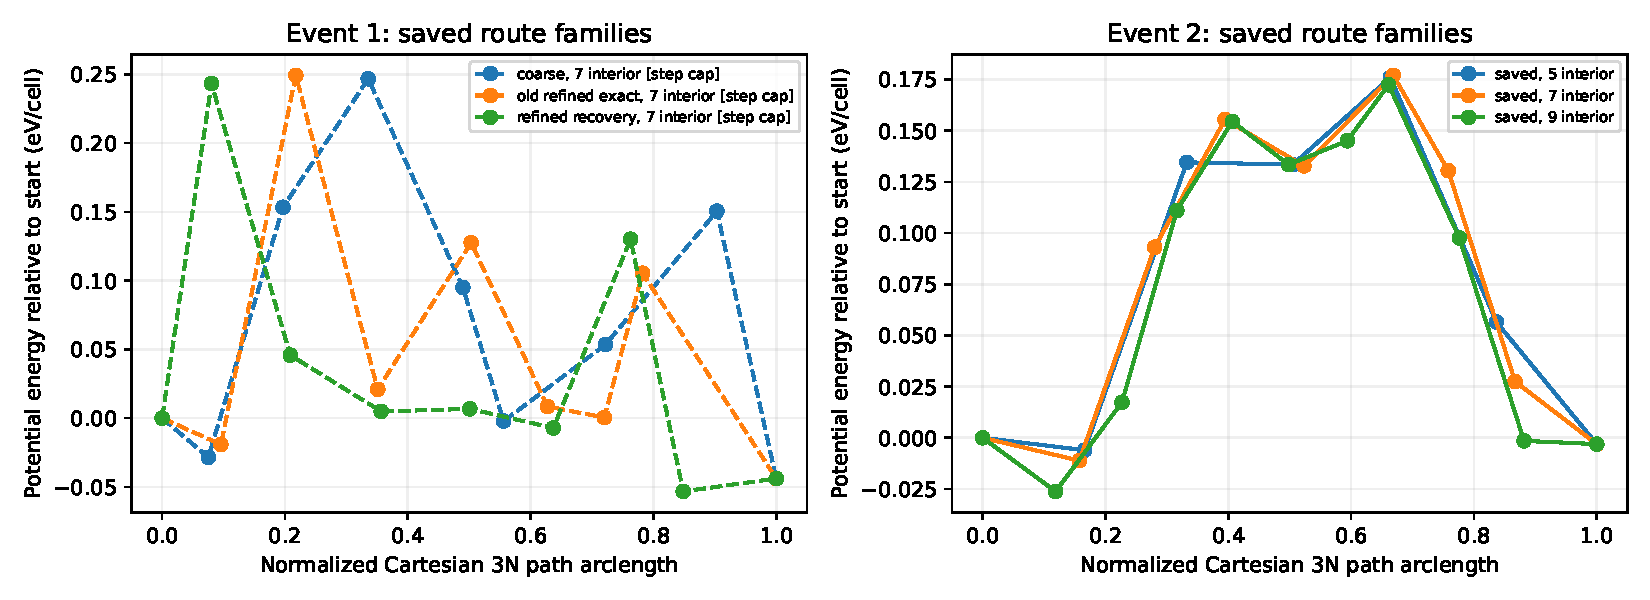
\includegraphics[width=.99\linewidth]{assets/route_profiles.pdf}\end{center}
Dashed profiles above are preserved terminal states of nonconverged event 1
calculations. The horizontal coordinate is normalized full-$3N$ Cartesian
arclength on the saved unwrapped branch, not a measured reaction time.

\subsection{A stable local unstable mode does not verify the complete hop}
The fixed-seven-image continuation reached the $0.01$~eV/\AA\ projected-force
target in 82 steps, with forward/reverse spans 0.16918/0.17231 eV. The forward
change from the 0.02 target is $-0.00784$~eV, within the declared numerical criterion.
The candidate climbing image 5 has physical maximum force 0.00888 eV/\AA.

Two central finite-difference Hessians use the \emph{same exact candidate}
at $\delta=0.01$ and 0.005\AA, with three fresh identical-coordinate force calls
before each. For 180 atoms, each full Cartesian Hessian costs 1,080 displaced force
calls. With $F_a=-\partial E/\partial R_a$,
\begin{equation}
H_{ab}\simeq-\frac{F_a(R+\delta e_b)-F_a(R-\delta e_b)}{2\delta}.
\end{equation}
$H$ is in eV/\AA$^2$. The mass-weighted matrix is $D=M^{-1/2}HM^{-1/2}$,
with atomic masses in amu. After symmetrization and removal of exactly three
translations, both 537-dimensional internal spectra have exactly one negative
eigenvalue: $-0.111003$/$-0.111010$~eV\,\AA$^{-2}$\,amu$^{-1}$. The next is
$+0.003343$; the two negative-mode vectors have absolute overlap 0.999999994.
Observed force-component repeat ranges are about $2.2\times 10^{-6}$~eV/\AA,
but these three-call ranges are not calibrated Hessian error bars. Independently
reconstructing both Hessians from the raw force pairs reproduces all eigenvalues;
all 2,160 displacement hashes and logged force maxima were checked.
Unweighted force-derivative noise and mass-weighted eigenvalues have different
units; their magnitudes are not directly compared. Displacement-size agreement
and mode overlap are the actual numerical evidence.

A negative curvature means displacement along that local mode lowers energy
to second order when the gradient is small. It does not identify the basins
reached farther away. The negative mode's absolute overlap with the actual ASE
improved tangent is 0.779 in the mass metric, or 0.920 when both are represented as
normalized Cartesian displacements. Those are different coordinate metrics,
not probabilities or independent physical replications.

These calculations produce MLIP potential-energy path spans in eV per marked
hop. They establish neither an activation free energy nor diffusivity. Later
physical validation needs endpoint/saddle/path DFT under compatible electronic
and spin settings. No VASP job or input deck is submitted during this goal.
\newpage

\subsection{Same raw vacancy mask, different continuous configurations}
The plus/minus negative-mode displacements were independently relaxed at a
$0.02$~eV/\AA\ maximum-force target. The minus branch is end-like: its
identity-preserving, host-aligned RMS difference from the original end is
0.04686\AA, with maximum atomic difference 0.06628\AA. The plus branch instead
reaches an off-site, force-small state: RMS 0.11671\AA\ and maximum difference
1.34843\AA\ from that same end. Its migrating Li is 1.5992\AA\ from its nearest
parent site, with only 0.05791\AA\ separating the first/second site distances.

\begin{center}\small
\begin{tabular}{lrrrr}\toprule
State&$E$ (eV/cell)&Li/site distance&4th O distance&5th O distance\\
& &\AA&\AA&\AA\\\midrule
Original end&$-1032.516551$&0.2562&2.1763&2.1806\\
Climbing image&$-1032.344237$&1.1984&2.3447&2.8548\\
Downhill minus&$-1032.521675$&0.2735&2.1684&2.1729\\
Downhill plus&$-1032.378428$&1.5992&1.9820&3.1853\\\bottomrule
\end{tabular}
\end{center}
The original end, climbing image, minus state and plus state all receive the
\emph{same raw nearest/Hungarian vacancy assignment}, hence the same orbit key,
despite these geometric and energy differences. The plus state has four nearer
O atoms, all within 1.982\AA, followed by a 1.203\AA\ gap to its fifth O; the minus
state has six O within 2.336\AA. These ranked distances require no unvalidated
bonding cutoff. Full periodic neighbors were searched within 5\AA\ only to obtain
the distance lists.

\begin{center}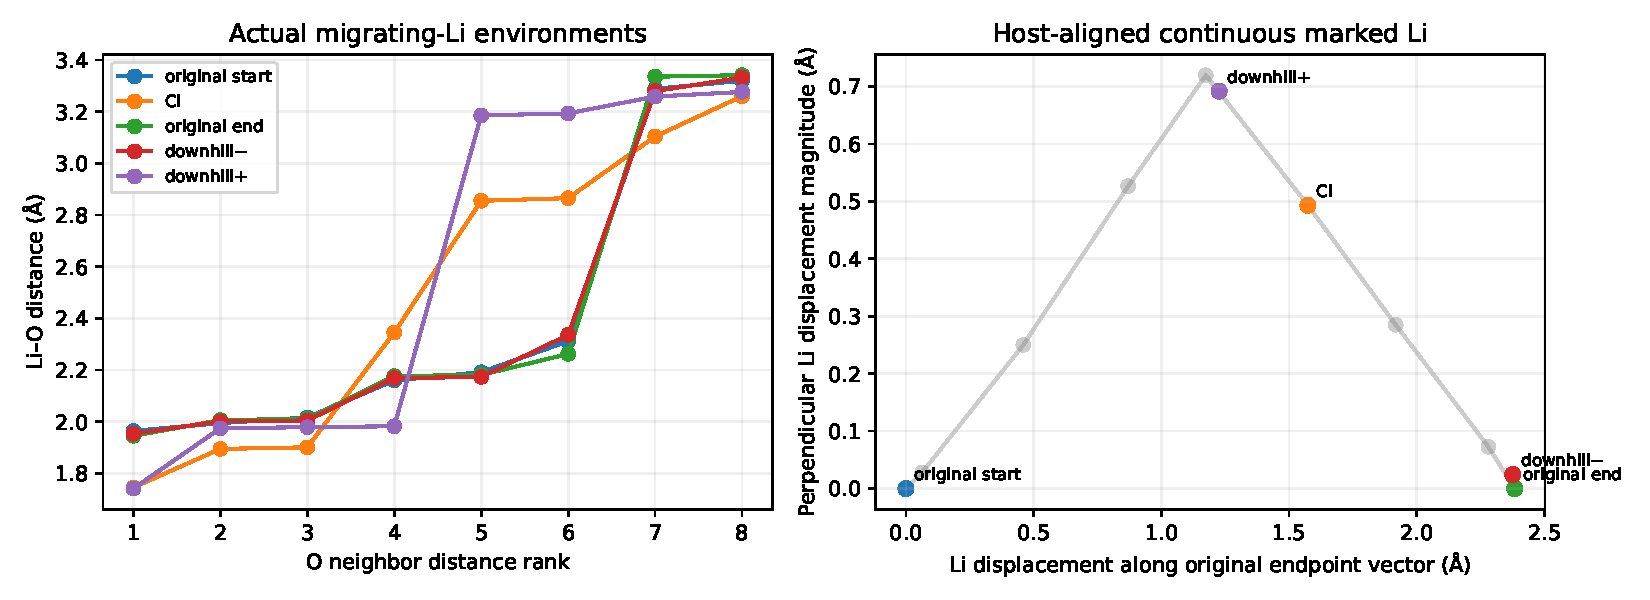
\includegraphics[width=.99\linewidth]{assets/candidate_environments.pdf}\end{center}
The right panel shows the actual continuous marked-Li geometry after removing
common host translation. The grey chain is the saved NEB route; perpendicular
displacement is a magnitude, not a signed plane coordinate. The off-site endpoint
is near an intermediate part of that route. This supports a possible compound
path with an intermediate state; neither its minimum character nor the complete
sequence of elementary connections has been certified. It does not invalidate a
protocol-defined pristine-mask-to-endpoint dataset, but it prevents using a
vacancy orbit as a unique continuous PES-basin identity.

On the unchanged original seven-image UMA path, MACE gives forward/reverse spans
0.16516/0.25159 eV and selects peak image 3 rather than UMA's 5. MACE endpoint
physical forces are 0.2567/0.2547 eV/\AA: these are not stationary MACE endpoints,
so the profile is not a MACE-optimized barrier. Independently tightening the same
original pair under each teacher defines a separate new-endpoint experiment.
\newpage

\subsection{Endpoint sensitivity prevents an overall stable-barrier claim}
Both original endpoints were independently tightened to $0.01$~eV/\AA\ under
each teacher, retaining the marked Li assignments. UMA lowered their energies
by 0.02151/0.000034~eV; MACE lowered them by 0.13892/0.10486~eV. Each new band kept
seven interior images and used the $0.02$~eV/\AA\ target. Initial interiors were
the original path plus a linear endpoint-displacement taper in its original
Cartesian arclength, with no quiet image resampling or new IDPP.

\begin{center}\small
\begin{tabular}{lrrrr}\toprule
New endpoints&Forward span&Reverse span&End minus start&Peak image\\
&eV&eV&eV&\\\midrule
UMA&0.195626&0.177294&$+0.01833$&5\\
MACE&0.199585&0.251953&$-0.05237$&3\\\bottomrule
\end{tabular}
\end{center}
The original fixed-seven-image $0.01$ case gave 0.169182~eV forward, while the
new UMA-endpoint band gives 0.195626~eV: a $+0.026444$~eV change, exceeding the
chosen 0.02~eV practical numerical target. Both endpoint coordinates and the band
force target differ in this comparison; it measures combined protocol
sensitivity, not an isolated endpoint-error contribution. The restricted
fixed-original image/tolerance comparison passed, but \emph{overall barrier
stability is not established}. A small force residual alone supplies no energy
error bound without information about local curvature.

The similar UMA/MACE forward heights are also insufficient: the reaction-energy
sign and highest-image identity differ, and the original marked path has not
been verified as one elementary hop. These are MLIP potential-energy path spans,
not validated activation free energies. No additional physics is run after this
bounded study; later DFT and fuller basin/connection verification remain necessary.

\section{Actual 537-mode harmonic null for the thermal estimator}
The earlier thermal work had a 21-mode synthetic check. The new check uses the
actual saved positive 537-mode spectrum and mass-weighted eigenvectors from one
180-atom basin. Three independent phase seeds generate nested 10/20/50 ps
synthetic velocity observations at 0.5 fs; each is analyzed by pinned ATLAS
py-xPT 2.1.0, commit\texttt{197bdcf5f57c9d04b5527f9e7d6f4fdb8bf3b82d}, under 1PT/2PT/3PT.
All 27 analyses completed without failures. An allocation auto-logout interrupted
the first attempt; its four complete results were reused immutably and its
incomplete raw output was preserved. No MLIP or MD calls were required.
\newpage

For mode $j$, frequency $\nu_j$ in THz(cycles/ps), normalized mass-weighted
eigenvector $Q_j$ and uniform phase $\phi_j$,
\begin{equation}
\dot q_j(t)=\sqrt{2 k_BT/C}\cos(2\pi\nu_jt+\phi_j),\qquad
v(t)=M^{-1/2}Q\dot q(t).
\end{equation}
$M$ is the diagonal mass matrix in amu; $C=1.0364269656262175\times 10^{-4}$
converts amu\,\AA$^2$/ps$^2$ into eV. Every mode has fixed total energy $k_BT$.
Random phases match canonical harmonic velocity second moments, but fixed modal
energies are not a canonical MD trajectory. The known harmonic Hamiltonian
nevertheless supplies an exact partition-function reference. The energy anchor
is $E_{\min}+537 k_BT$ and is included once. Only 3 COM modes are excluded;
no separate molecular rotations/translations are subtracted from the crystal.

Finite windows have a slightly shifted observed kinetic temperature. We compare
entropy at that native temperature and explicitly match the supplied total-energy
anchor rather than interpreting a first-order temperature transport as exact.
If $\mathcal E$ is that anchor and $S_h,U_h$ are exact harmonic quantities,
\begin{align}
F_{\rm c,ref}&=\mathcal E-TS_{\rm c,h},\\
F_{\rm q,ref}&=\mathcal E+[U_{\rm q,h}-(E_{\min}+537 k_BT)]-TS_{\rm q,h}.
\end{align}
At the target temperature these reduce to the usual classical/quantum harmonic
free energies. At the observed temperature they isolate estimator error from
the known finite-window anchor mismatch.

\begin{center}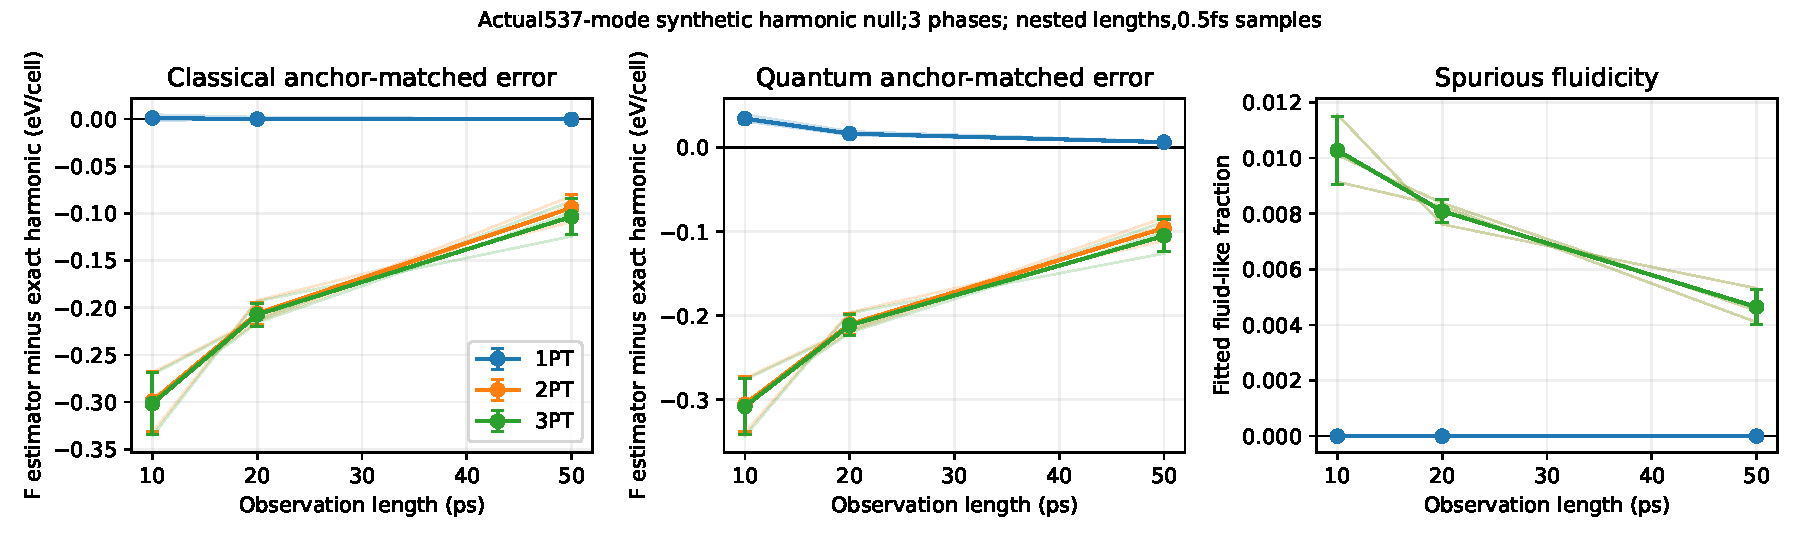
\includegraphics[width=.99\linewidth]{assets/harmonic_null_bias.pdf}\end{center}
The mean 1PT quantum anchor-matched error decreases from about+0.0344 eV/cell
at 10 ps to+0.00645 at 50 ps. In contrast, 2PT/3PT infer nonzero fluidicity
0.0041--0.0116 from an analytically bounded harmonic signal with no diffusion.
At 50 ps, 3PTquantum errors range from$-0.0884$ to$-0.1260$eV/cell across phases.
Longer windows help, but do not establish convergence at these lengths.

COM speeds are numerically negligible; energy-anchor round trips are exact,
$F=U-TS$ residuals are at floating-point roundoff, and the integrated spectrum
contains 537 modes to within about$1.2\times 10^{-6}$modes. Correct mode
normalization alone therefore does not imply a correct free-energy estimate.
Phase spread is descriptive, and nested lengths are correlated. This is a
harmonic estimator null, not an anharmonic correction, an unrestricted equilibrium
MD result or validation of real-LCO thermodynamics. Discrete vacancy entropy and
within-basin vibrational entropy cannot simply be added without a consistent
basin partition, energy convention and statistical measure.

\clearpage\section*{Evidence, execution and later physical validation}
Raw small-cell labels, per-geometry hashes, stored representative masks,
teacher/precision receipts and finite-model tables are in
\texttt{reports/overnight\_20261108/smallcell}. Independent arithmetic and literal
geometry checks are in\texttt{smallcell\_independent\_v2}. A first checker failure
was retained: its roundoff scale incorrectly used a small energy difference
rather than the magnitudes of the subtracted energies. The repaired arithmetic
bound uses the same 128 machine-epsilon factor with the operand scale; no
scientific label or result changed. The independent check verifies 1,364 geometries
and 11,104 numeric fields, with maximum difference$2.84\times 10^{-13}$.

NEB inputs, full physical/projected forces, continuous parent atom IDs,
unconverged routes, actual call logs and scheduler interruption evidence are
retained. Harmonic raw spectra/configuration/native results, deterministic phases,
input Hessian/minimum hashes and the reused-result lineage remain available.
The new condition schemas explicitly state or link authoritative FP32/TF32-off
inference receipts; old-schema omissions are not treated as evidence of wrong
inference.

The later-DFT geometry handoff contains the candidate, both original endpoints,
both downhill states and every intermediate band image as exact-coordinate NPZ
with original same-geometry UMA energy/force/stress labels, plus POSCAR/CIF viewing
exports. Local-to-parent atom IDs, source/checkpoint hashes and coordinate hashes
are preserved. The off-site plus state is explicitly retained as an example of
the limitations of a vacancy-only representation; it is not silently merged with
the end-like state sharing its assigned mask.

Exact commands and final allocation/cost/publication receipts belong to the
integrated goal packet. New code is under
\texttt{scripts/overnight\_20261108}; no new allocation is requested by these
analysis scripts. Model weights are not redistributed. Resource accounting
distinguishes allocated node time, GPU-device time, actual static E/F calls,
relaxations and analysis work; final totals are attached after job release.

Ricardo should inspect physical paths, endpoint residuals and teacher disagreement
before selecting later DFT candidates. Beihao's class task remains independent
model-mechanism verification, not demonstrating a physical entropy/barrier claim.
Varad should independently replay raw probabilities, multiplicities, repeated
queries, failed attempts and costs. A stable same-MLIP result still needs later
DFT and experimental comparison before a physical recycling conclusion.

\bibliographystyle{unsrt}\bibliography{references}
\end{document}
